% -------------------------------------------------------------------
% - NAME:        poster.tex
% - AUTHOR:      Reto Stauffer
% - BASED ON:    Jakob Messners version of this theme
% - DATE:        2014-09-29
% -------------------------------------------------------------------
% - DESCRIPTION: This is a demo template for portrait beamer poster
%                in the UIBK design 2017.
% -------------------------------------------------------------------
\documentclass[final]{beamer} 

%\usepackage[orientation=portrait,size=a0,scale=1.30]{beamerposter}
%\usetheme[ncols=2]{uibkposter}
%% ------------------------------------------------------------------
%% Use the two lines above for portrait posters
%% ------------------------------------------------------------------

\usepackage[orientation=landscape,size=a1,scale=1.30]{beamerposter}
\usetheme[ncols=3,orangetheme]{uibkposter}
\usepackage{subcaption}
\usepackage[font={tiny}]{caption}
\usepackage{ragged2e} 
%% ------------------------------------------------------------------
%% Use the two lines above for landscape posters
%% The option 'orangetheme' can be used to switch the theme.
%% Additional options allowed:
%% - orangetheme: uses alternative color theme
%% ------------------------------------------------------------------

\headerimage{1}
%% ------------------------------------------------------------------
%% The theme offers four different header images based on the
%% corporate design of the university of innsbruck. Currently
%% 1, 2, 3 and 4 is allowed as input to \headerimage{...}. Default
%% or fallback is '1'.
%% ------------------------------------------------------------------

%% ------------------------------------------------------------------
%% The official corporate colors of the university are predefined and
%% can be used for e.g., highlighting something. Simply use
%% \color{uibkorange} or \begin{color}{uibkorange} ... \end{color}
%% Defined colors are:
%% - uibkorange, uibkblue, uibkgray, uibkgraym
%% Please note that there are two faculty colors (see definition above)
%% - uibkcol, uibkcoll
%% The frametitle color can be easily adjusted e.g., to black with
%% \setbeamercolor{titlelike}{fg=black}
%% ------------------------------------------------------------------

%\setbeamercolor{verbcolor}{fg=uibkorange}
%% ------------------------------------------------------------------
%% Setting a highlight color for verbatim output such as from
%% the commands \pkg, \email, \file, \dataset 
%% ------------------------------------------------------------------

%% The title of your poster
\title{The Cradle of Asymmetric Cryptography}

%% If the subtitle is not set or empty no subtitle will be shown
\subtitle{Secure Communications Over Insecure Channels}

%% Author(s) of the poster
\author{Kristina Magnussen} 

%% Enable numbered captions (figures, tables)
\setbeamertemplate{caption}[numbered]

\usepackage{tikz} %% For the example figure

%% Begin document
\begin{document}

\begin{frame}[fragile]
\begin{columns}[t]

%% ------------------------------------------------------------------
%% This template contains content for both, the portrait version (two
%% columns) and the landscape version (three columns).
%% If \usepackage[orientation=portrait,...]{beamerposter} then the
%% center column is unused (only left and right column). In this
%% case simply remove the block:
%%     \if@beamerposter@portrait
%%         [...]
%%     \fi
%% If \usepackage[orientation=landscape]{beamerposter} the layout 
%% comes with three columns (left, center, right). In this case
%% remove the \if@beamerposter@portrait, \else and \fi condition but
%% keep the block:
%%     \begin{centercolumn}
%%         [...]
%%     \end{centercolumn}
%% ------------------------------------------------------------------

%% ------------------------------------------------------------------
%% begin left column for both, portrait and landscape
%% ------------------------------------------------------------------
\begin{leftcolumn}
   %% please leave one blank line here

   %% first block
   \begin{boxblock}{Motivation}
   	\justifying
   	 \begin{alertblock}{Some Historical Background}
   	 	\justifying
   		   	Ralph Merkle developed \textbf{Merkle's puzzles} in \textbf{1974} for a university project. The idea was rejected by his professor. At this time, asymmetric cryptography concepts were not known to the public. 
   	\end{alertblock}

     \begin{itemize}
     	\item Symmetric crypto requires key exchange \\ $\rightarrow$ additional \emph{secure channel} needed to transmit key
     	\item This new method allows communication partners to transmit a key over \emph{insecure channels} 
     	\item \emph{Assumption:} Attacker can read everything sent on this channel
     	\item \emph{Advantages of this method:}
     	\begin{itemize}
     		\item Solution to key distribution problem
     		\item Easier key exchange in network with multiple communication partners 
     	\end{itemize}
     \end{itemize}

   \end{boxblock}

   %% second block

   %% Third block
   \begin{boxblock}{Puzzle Creation}
   	\justifying
   	\begin{block}{Definition}
   			\justifying
   	\textbf{Puzzle:} Cryptogram which can be solved through cryptanalysis \\ $\rightarrow$ Puzzle is meant to be \emph{solved}.
   	\end{block}
 
   	\begin{itemize}
   		\item \emph{Idea:} Hide information (here the secret key) in a puzzle by encrypting it
   		\item Restricting the key space keeps puzzle solvable \\ $\rightarrow$ Increase/decrease puzzle difficulty by adapting key space
   	\end{itemize}
   	
   	\begin{figure}
   		\begin{subfigure}{0.95\textwidth}
   			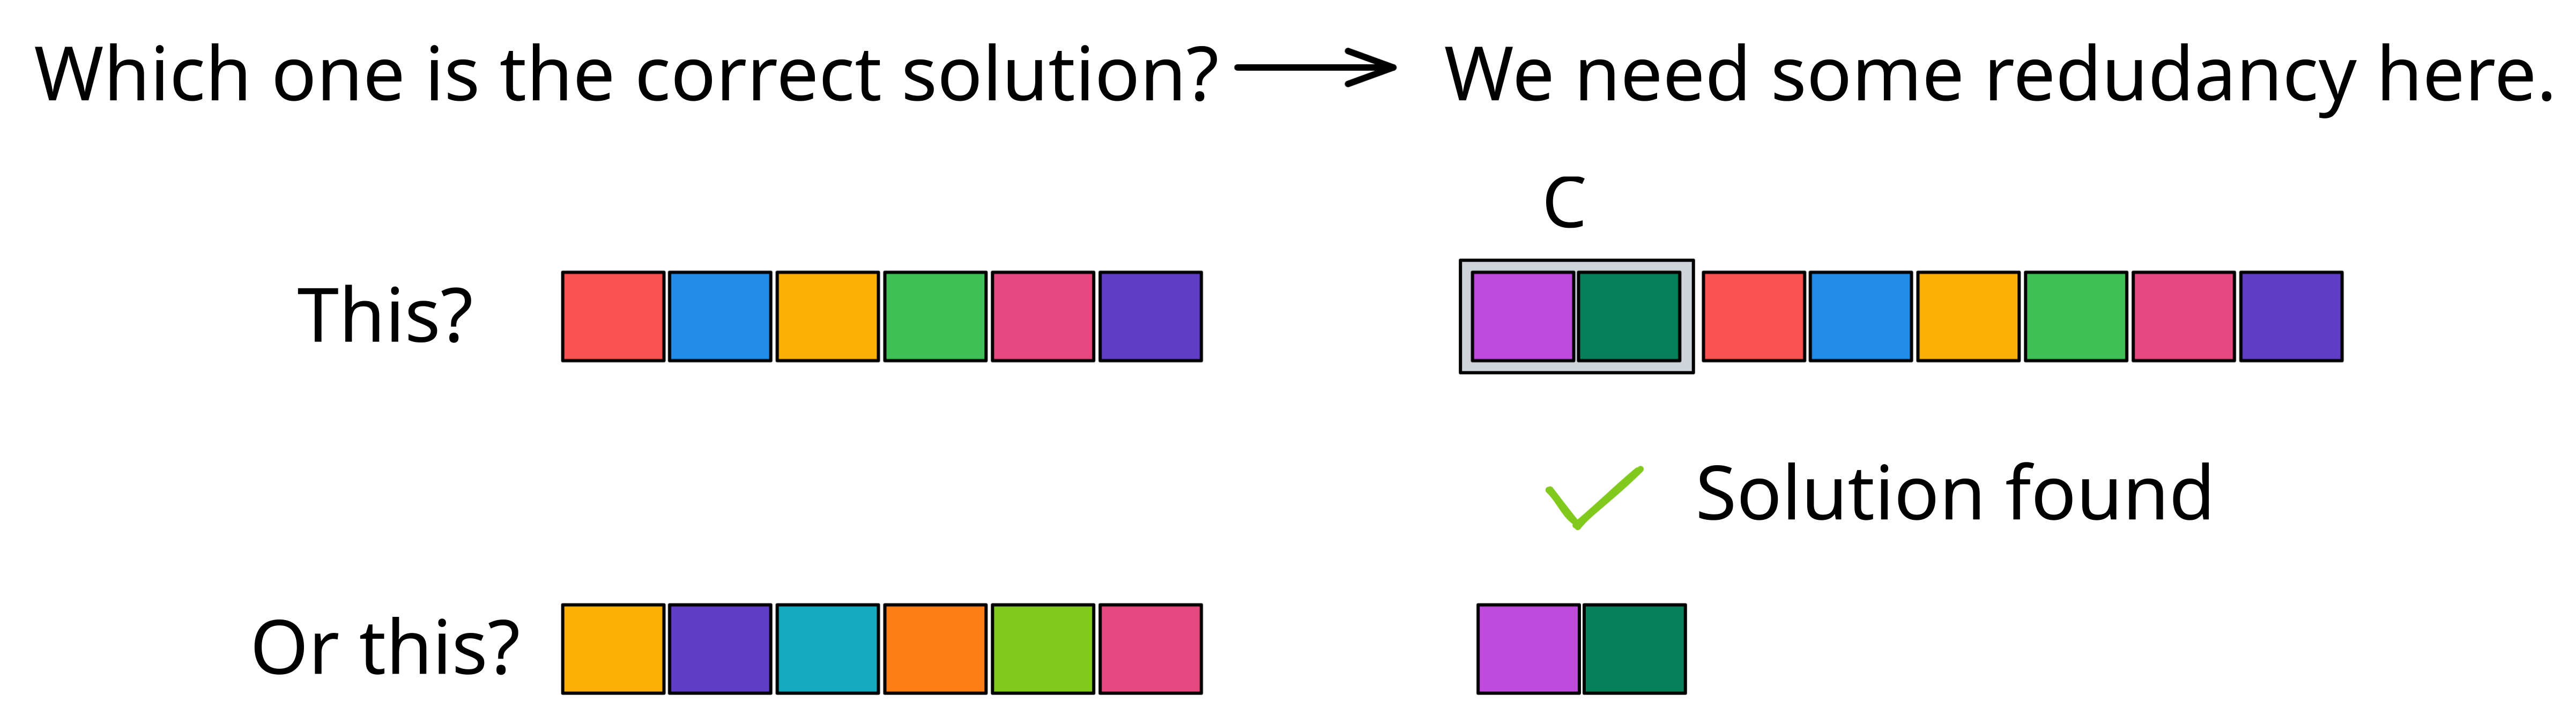
\includegraphics{Random_new.png}
   			\vspace{0.1cm}
   			\caption{Constant C introduces redundancy to make the puzzle solvable and is communicated in plain text.}
   		\end{subfigure}
   	    \begin{subfigure}{0.53\textwidth}
   		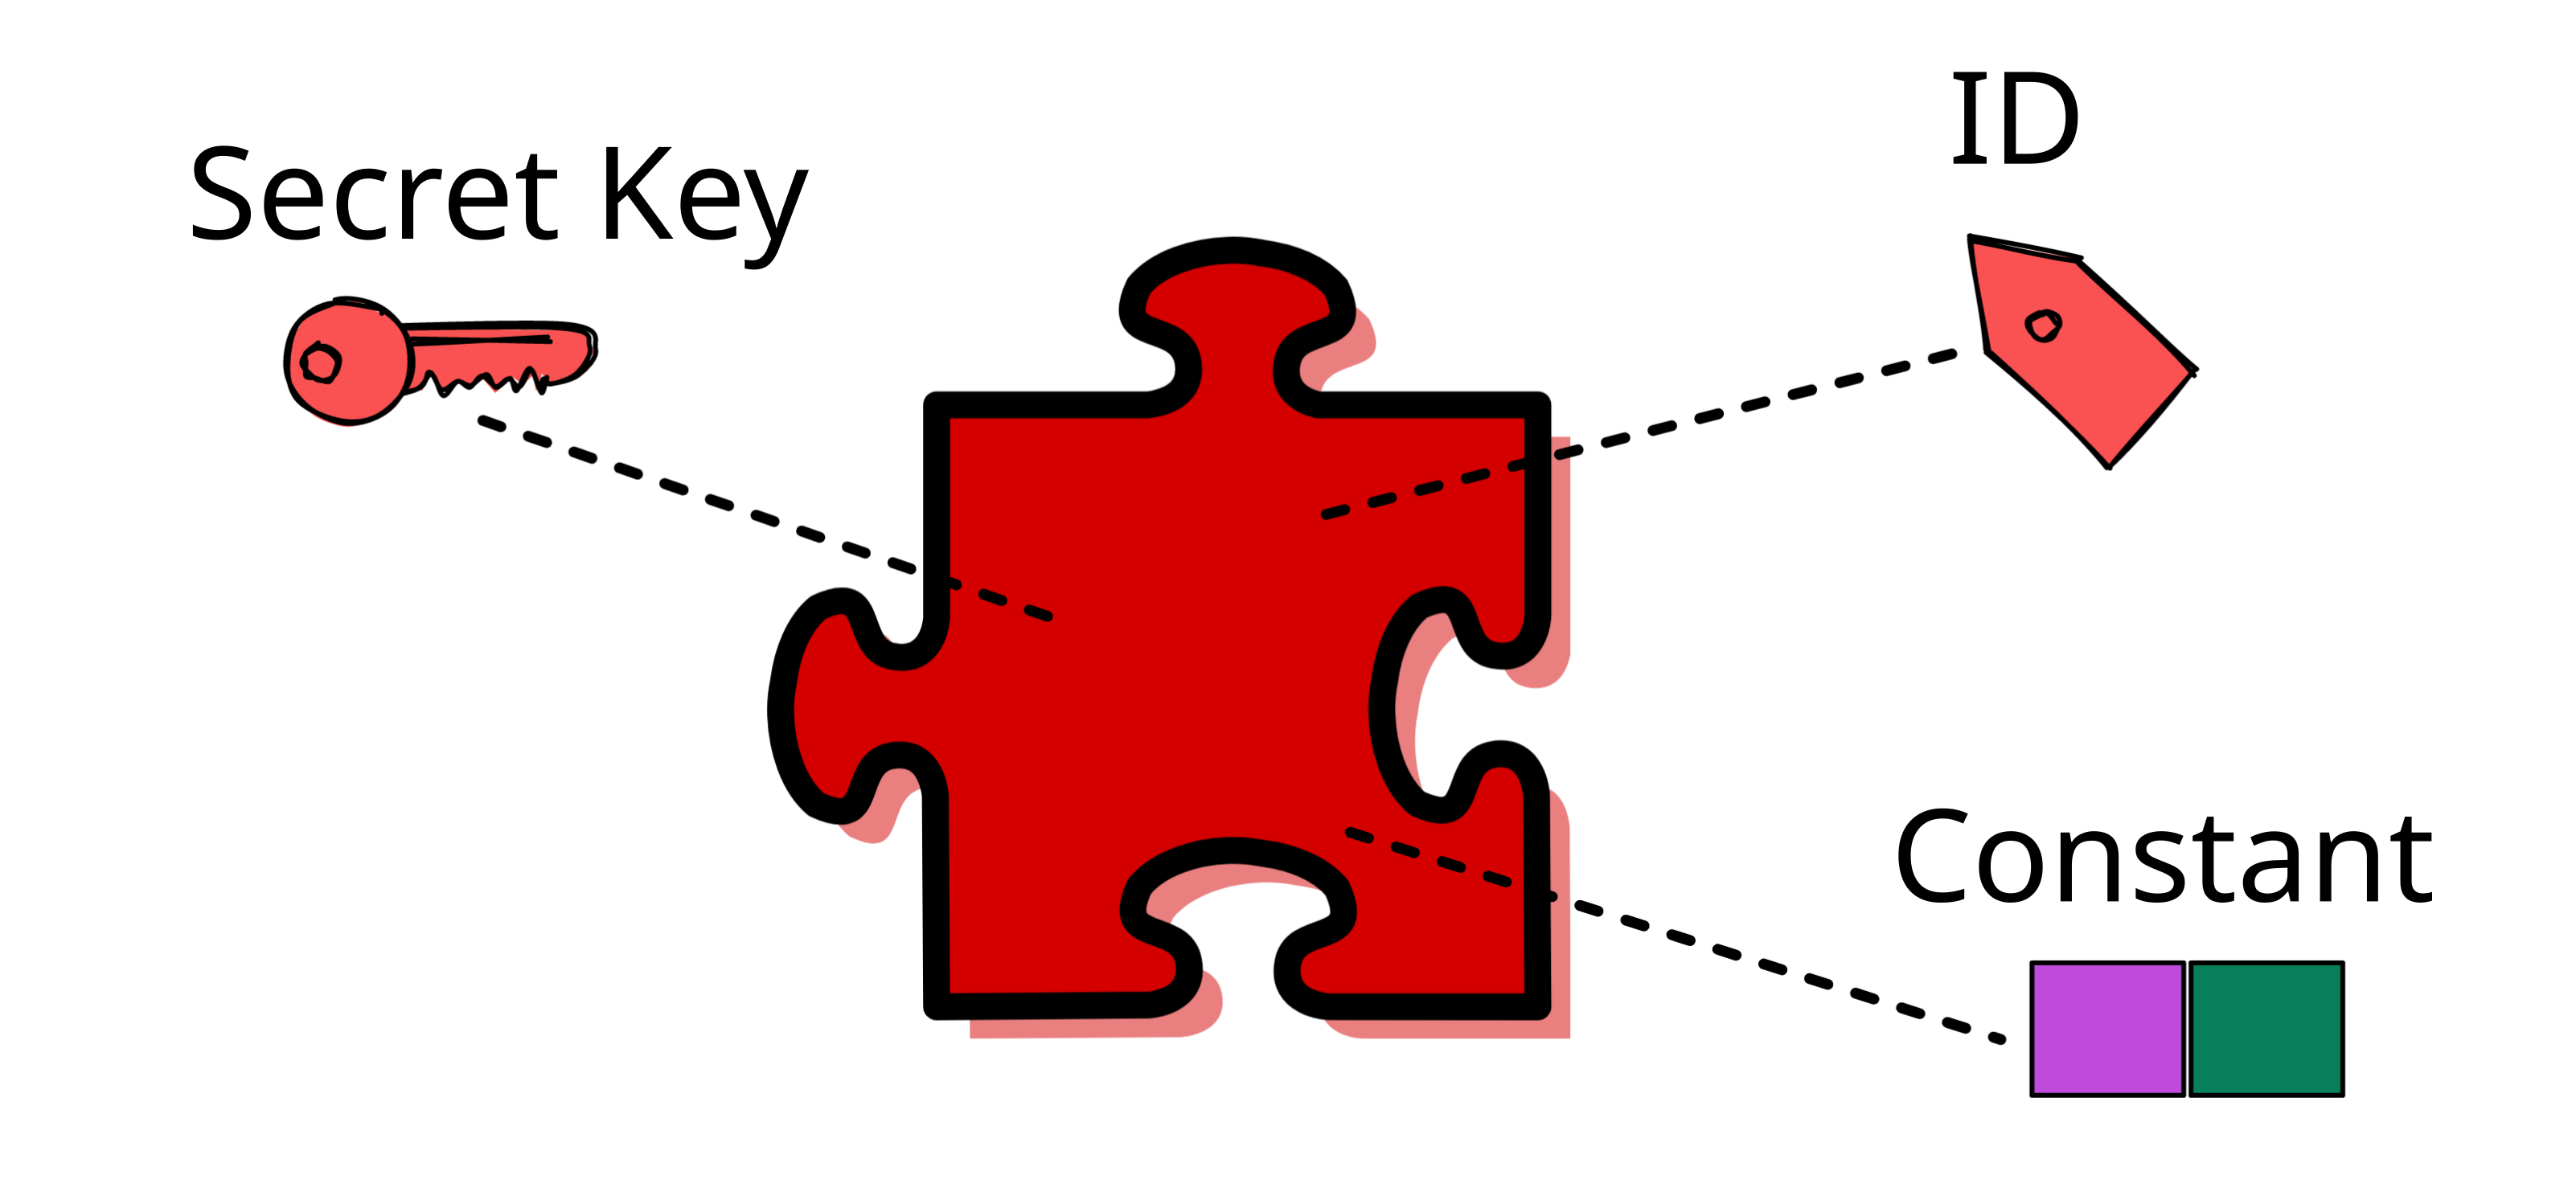
\includegraphics{Puzzle_struct_new.png}
   		\vspace{0.1cm}
   		\caption{Information contained in the puzzle.}
   	\end{subfigure}
   	\end{figure}
 

  

      
   \end{boxblock}

\end{leftcolumn} %% end left column


%% ------------------------------------------------------------------
%% This \if\else\fi statement is only for the template.
%% ------------------------------------------------------------------
\iflandscape
   %% ---------------------------------------------------------------
   %% Begin center column (for landscape only)
   %% ---------------------------------------------------------------
   \begin{centercolumn}
      %% please leave one blank line here

 

      \begin{boxblock}{Key Exchange using Puzzles}
         \begin{figure}
              \vspace{0.05cm}
             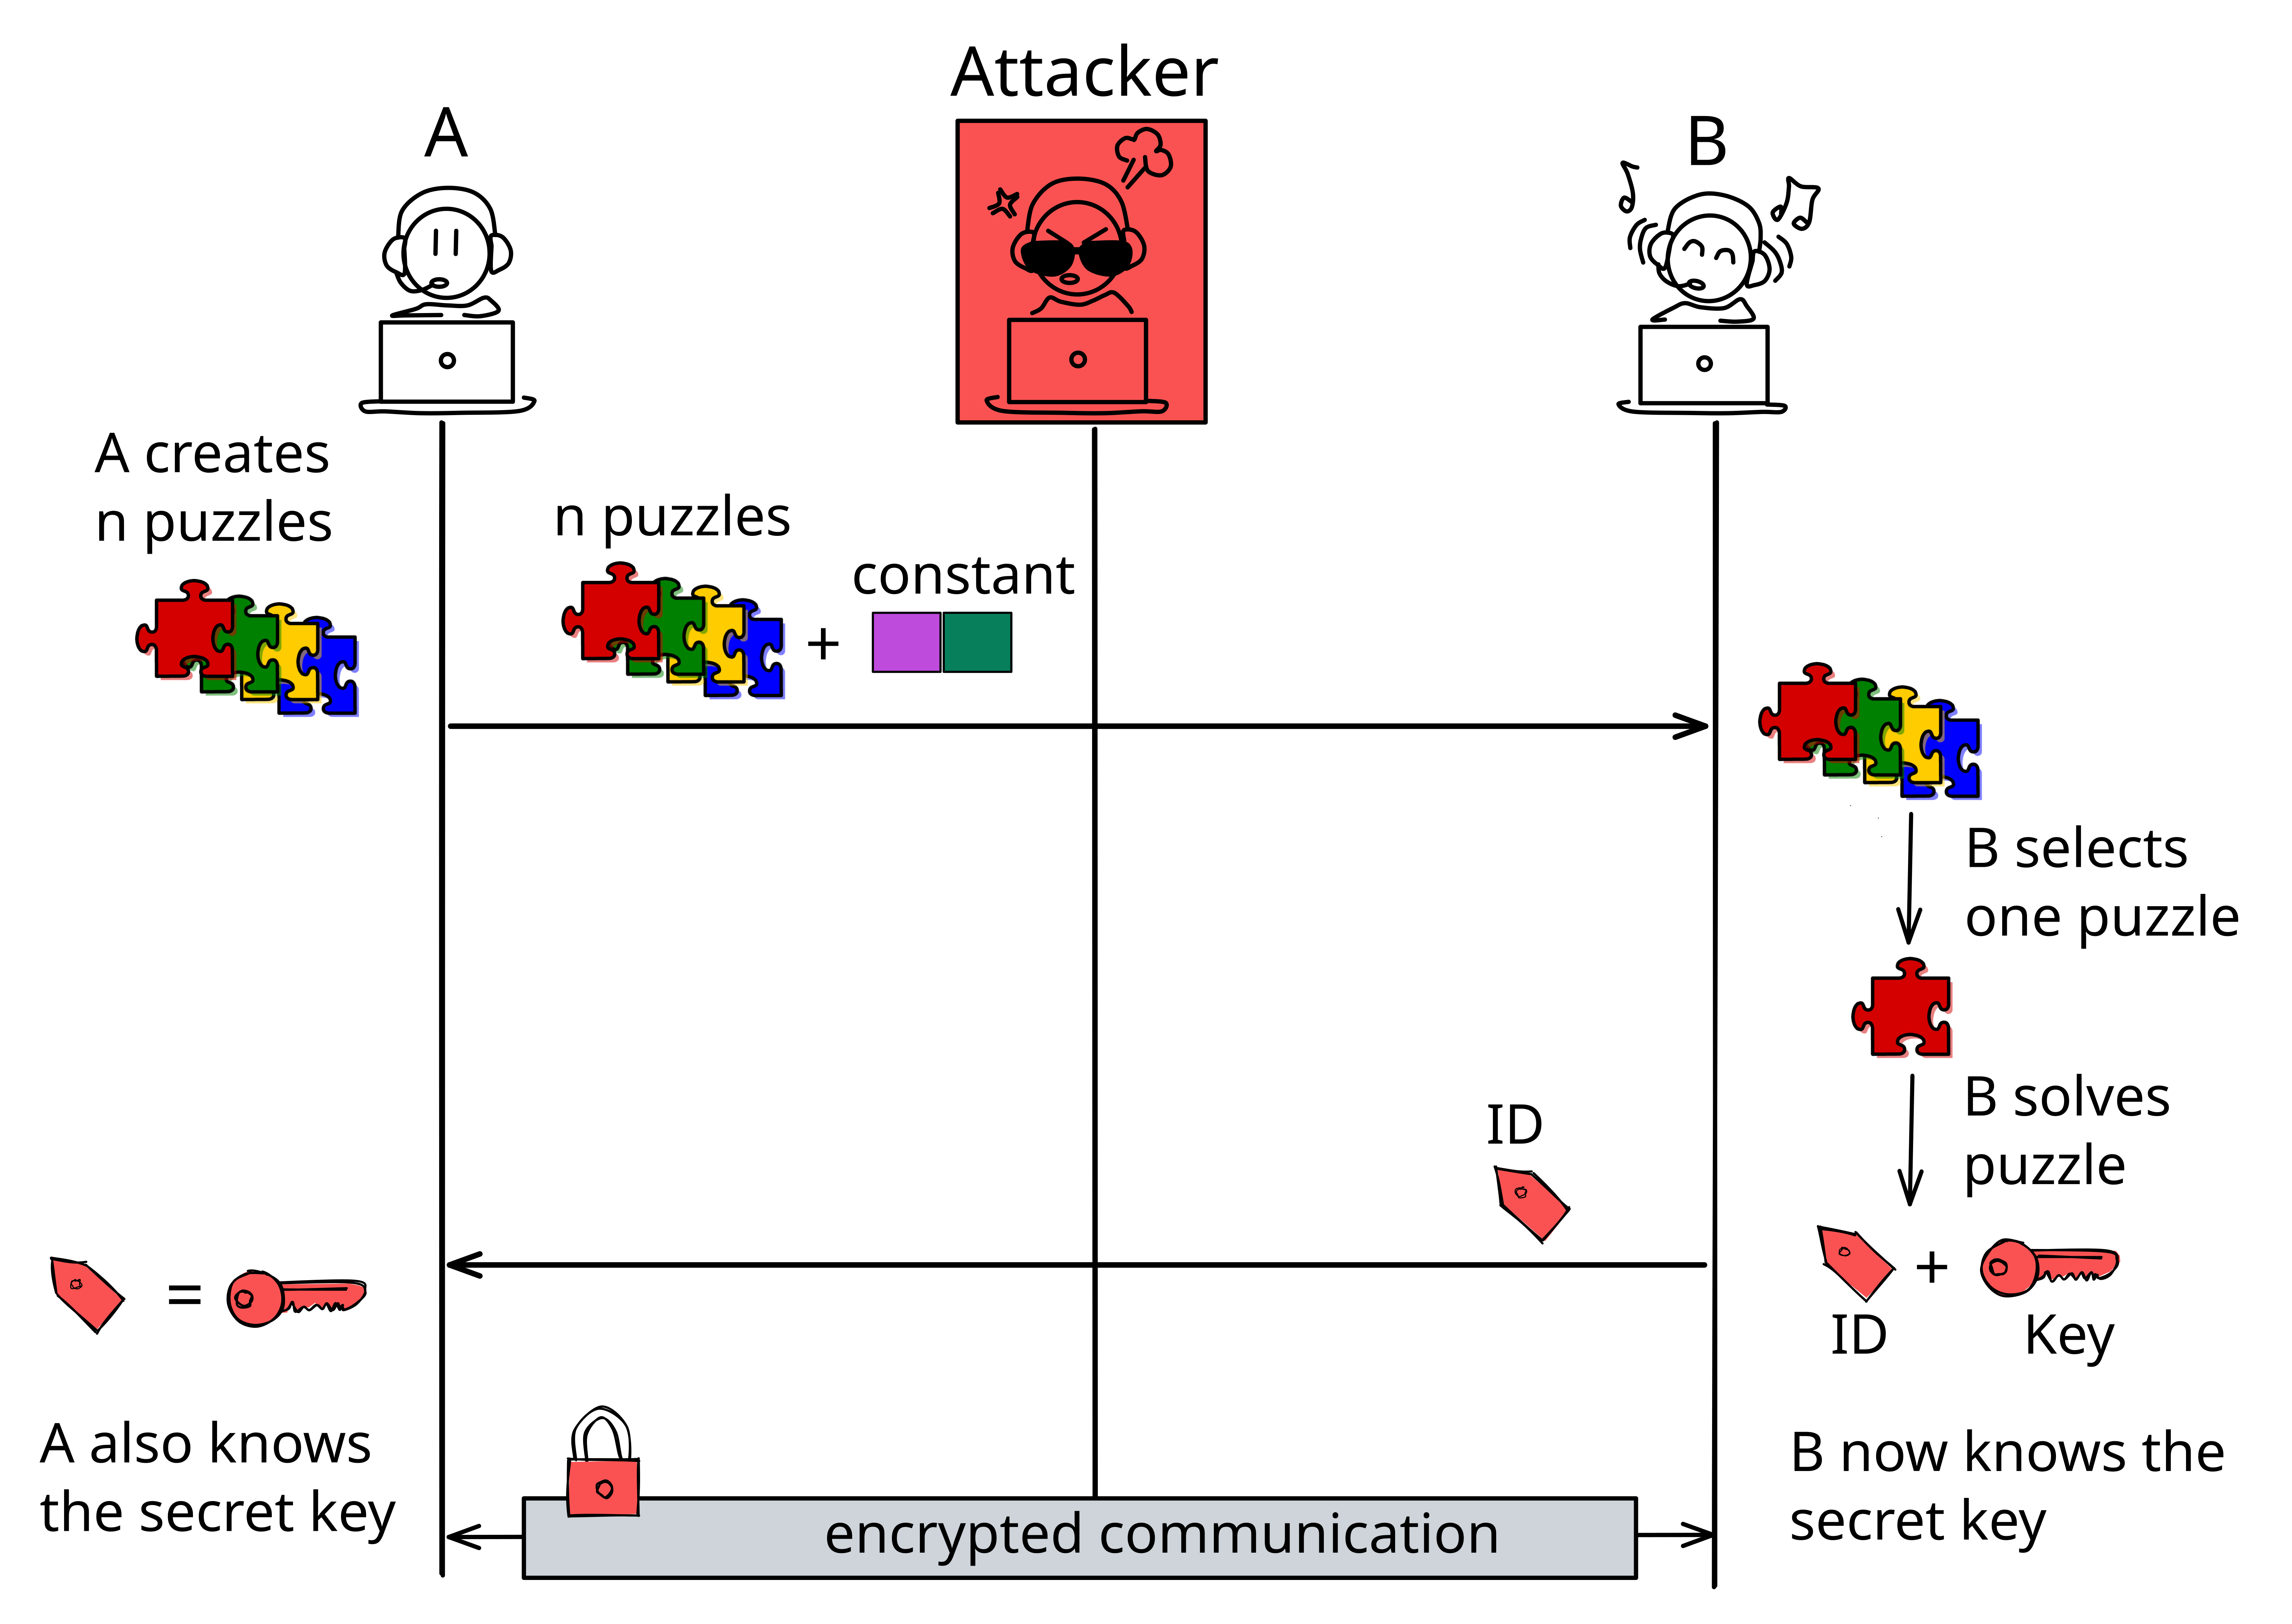
\includegraphics{sequence_new.png}
             \vspace{0.5cm}
            \caption{This sequence diagram shows the key exchange between two communication partners A and B using puzzles. The first two messages are unencrypted.}
         \end{figure}

      \end{boxblock}
  
       \begin{boxblock}{Security of Merkle's Puzzles}
  	\justifying
  	\begin{figure}
  		\centering
  		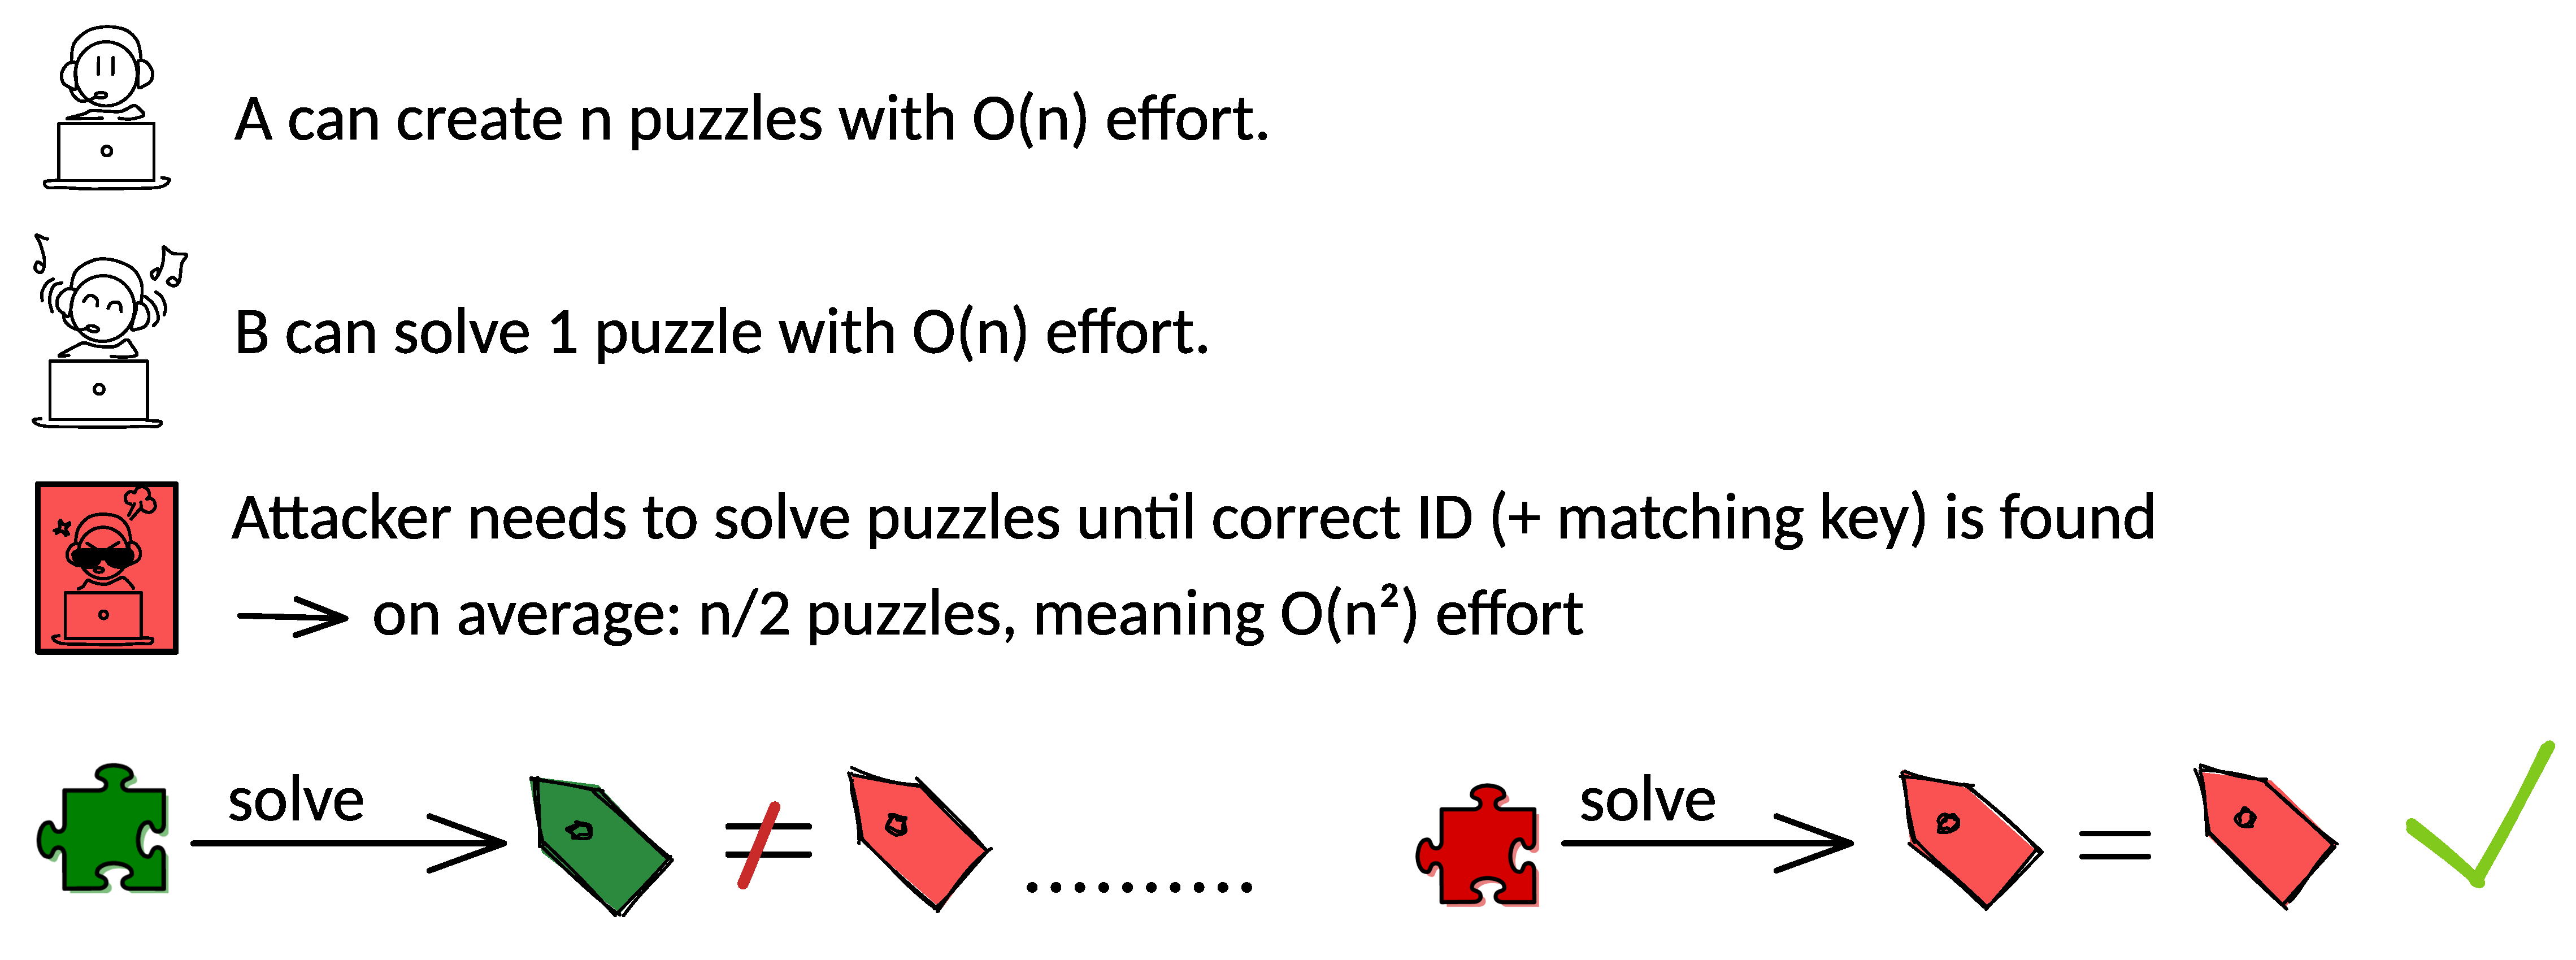
\includegraphics{attacker_view_new.pdf}
  		\vspace{0.4cm}
 
  	\end{figure}
   \begin{alertblock}{What Does This Mean for Security?}
   		\justifying
  	Even if a large $n$ is chosen, attacker only has to put in $O(n^2)$ effort, which makes brute-force attacks feasible.  \\
  \end{alertblock}
\vspace{0.36cm}
\begin{exampleblock}{Example}
	\justifying
	For $n=10 000$, the attacker has to calculate $5000$ puzzles on average. If it takes about 1 minute to solve a puzzle, the attacker will have found the key in about $3.5$ days.
\end{exampleblock}
  
  
  
  
  	
  \end{boxblock}



   \end{centercolumn} %% end center column
\fi


%% ------------------------------------------------------------------
%% begin right column for both, portrait and landscape
%% ------------------------------------------------------------------
\begin{rightcolumn}
   %% please leave one blank line here
   
   \begin{boxblock}{Disadvantages}
   	\justifying
   	\begin{itemize}
   		\item For exchanging a key, communication partners have to transmit a large amount of data
   		\item The larger the \emph{n}, the larger the amount of effort communication partners have to expend \\
   		$\rightarrow$ A moderate amount of security requires a very large \emph{n}. 
   	\end{itemize}
   	\end{boxblock}

   \begin{boxblock}{Merkle's Method Compared to Current Asymmetric Schemes}
\justifying
     	\begin{block}{State of the Art Asymmetric Encryption Schemes}
     			\justifying
     	Current asymmetric encryption schemes are based on problems which are considered to be \textbf{mathematically hard} to solve. \\ 
     	$\rightarrow$ Computing these problems is \emph{infeasible} for  large values. \\
     \end{block}
	Asymmetric Encryption Schemes are mainly based on:
     		\begin{itemize}
     			\item \emph{Discrete Logarithm Problem}
     			\item \emph{Integer Factorization Problem}. 
     		\end{itemize}
   
        
        
%        \begin{exampleblock}{Diffie-Hellmann}
%          Key exchange algorithm based on the \emph{Discrete Logarithm Problem}.
%        \end{exampleblock}
%   

        
     
%     
%         \begin{table}
%         \begin{tabular}{l l l l}
%            \hline
%             & Merkle's Puzzles & Diffie-Hellman & RSA \\
%            \hline \hline
%             Performance     &  \fct{example} \\
%            \verb|\class{...}|   &  \class{example} \\
%            \verb|\pkg{...}|     &  \pkg{example} \\
%            \verb|\email{...}|   &  \email{email} \\
%            \verb|\doi{...}|     &  \doi{example} \\
%            \verb|\file{...}|    &  \file{example} \\
%            \verb|\dataset{...}| &  \dataset{example} \\
%            \hline
%         \end{tabular}
%         \caption{Commands provided by the \class{beamerstyleuibk} template.}
%         \end{table}


 

   \end{boxblock}

   %% Last block
   \begin{boxblock}{Lessons Learned}
 
 \justifying
      	\begin{alertblock}{Influence of Merkle's Puzzles}
      			\justifying
      		The rejected idea of a student became one of the first \emph{public-key protocols} known to the public. 
      	\end{alertblock}
      
      \begin{itemize}
      	\item Merkle's idea inspired the \emph{Diffie-Hellmann} key exchange, which is still widely used today.
      	\item The original idea does not offer a sufficient level of security, however, the idea could serve as a base for other protocols.
         
      \end{itemize}
      
      
   \end{boxblock}

   %% References
   \begin{footnotesize}
   
   \vspace{0.3cm}
   \begin{minipage}[t]{0.75\textwidth}
      \textbf{References:} \\
      %\bibliographystyle{ametsoc}
      %\bibliography{EMS}
      R. C. Merkle. Secure communications over insecure channels. Communications of the ACM, 21(4):294–299, 1978 \\
      C. Paar \& J. Pelzl (2010): Understanding Cryptography, Springer \\
      http://www.merkle.com/1974/

      \vspace{1cm}
   
   \end{minipage}
   \hfill
  
   \end{footnotesize}
\end{rightcolumn}
%% end right column %%%%%%%%%%%%%%%%%%%%%%%%%%%%%%%%%%%%%%%%%%%%%%%%%%
%%%%%%%%%%%%%%%%%%%%%%%%%%%%%%%%%%%%%%%%%%%%%%%%%%%%%%%%%%%%%%%%%%%%%%
%%%%%%%%%%%%%%%%%%%%%%%%%%%%%%%%%%%%%%%%%%%%%%%%%%%%%%%%%%%%%%%%%%%%%%
%%%%%%%%%%%%%%%%%%%%%%%%%%%%%%%%%%%%%%%%%%%%%%%%%%%%%%%%%%%%%%%%%%%%%%

\end{columns}
\end{frame}

\end{document}
